\documentclass[tikz,border=2pt]{standalone}
\usepackage{amsmath,amssymb}
\usepackage{tikz}
\usepackage{pgfplots}
\pgfplotsset{compat=1.18}

\begin{document}
% Normal demand approximation for meals: mu = 100, sigma = 20, beta = 0.6; the shaded left
% tail has probability 0.6 and ends at y* = mu + sigma Phi^{-1}(0.6) = 100 + 20 x 0.2533 = 105.07.
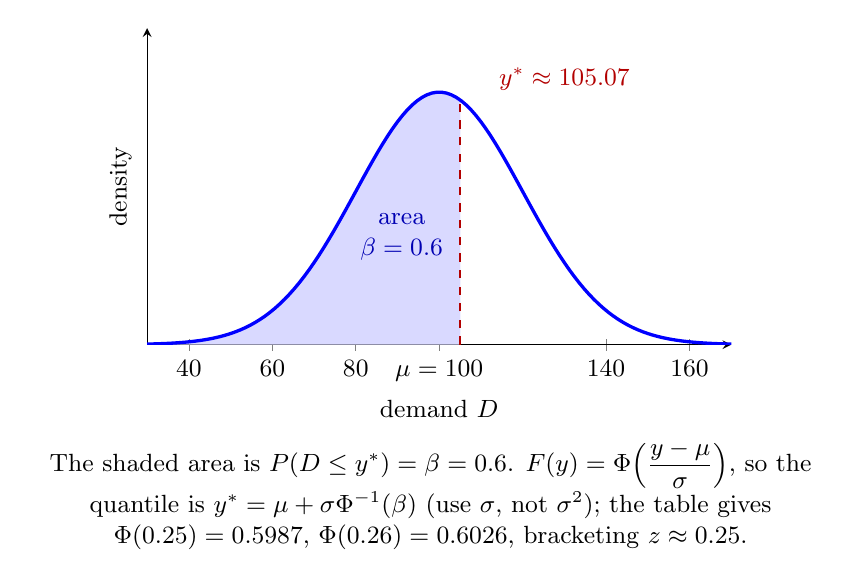
\begin{tikzpicture}
	\begin{axis}[width=9cm, height=5.6cm, xlabel={demand $D$}, ylabel={density}, xmin=30, xmax=170, ymin=0, ymax=0.025, axis lines=left, tick label style={font=\small}, label style={font=\small}, xtick={40,60,80,100,140,160}, xticklabels={40,60,80,$\mu=100$,140,160}, ytick=\empty, samples=120]
		\addplot[fill=blue!15, draw=none, domain=30:105.07] {exp(-((x-100)/20)^2/2)/(20*sqrt(2*pi))} \closedcycle;
		\addplot[blue, very thick, domain=30:170] {exp(-((x-100)/20)^2/2)/(20*sqrt(2*pi))};
		\draw[red!70!black, dashed, thick] (axis cs:105.07,0) -- (axis cs:105.07,0.0193);
		\node[font=\small, blue!70!black, align=center] at (axis cs:91,0.0085) {area\\ $\beta=0.6$};
		\node[anchor=west, font=\small, red!70!black] at (axis cs:112,0.021) {$y^*\approx105.07$};
	\end{axis}
	\node[anchor=north, align=flush center, text width=10cm, font=\small] at (3.6,-1.1) {The shaded area is $P(D\le y^*)=\beta=0.6$. $F(y)=\Phi\!\left(\dfrac{y-\mu}{\sigma}\right)$, so the quantile is $y^*=\mu+\sigma\Phi^{-1}(\beta)$ (use $\sigma$, not $\sigma^2$); the table gives $\Phi(0.25)=0.5987$, $\Phi(0.26)=0.6026$, bracketing $z\approx0.25$.};
\end{tikzpicture}
\end{document}
